\documentclass{article}
\usepackage{amsmath,amsfonts,booktabs,stmaryrd,tabularx,multirow,xfrac,nicematrix}
\usepackage{ltablex}
\usepackage{tikz}
\usetikzlibrary{decorations.pathmorphing,calc,positioning}
\usepackage{imakeidx}
\makeindex
\def\indexx#1{\index{#1}#1}
\usepackage{geometry}

\usepackage{amsmath,amsthm}
\newtheorem{definition}{Definition}

\usepackage{todonotes}
\setuptodonotes{inline}

\def\version{0.1.0}
\def\ebicommandlist{\begin{itemize}
\item\texttt{Ebi analyse completeness} or \texttt{Ebi ana comp}
\item\texttt{Ebi analyse medoid} or \texttt{Ebi ana med}
\item\texttt{Ebi analyse minimum-probability-traces} or \texttt{Ebi ana minprob}
\item\texttt{Ebi analyse most-likely-traces} or \texttt{Ebi ana mostlikely}
\item\texttt{Ebi association all-trace-attributes} or \texttt{Ebi asso atts}
\item\texttt{Ebi association trace-attribute} or \texttt{Ebi asso att}
\item\texttt{Ebi conformance entropic-relevance} or \texttt{Ebi conf er}
\item\texttt{Ebi conformance jensen-shannon} or \texttt{Ebi conf jssc}
\item\texttt{Ebi conformance jensen-shannon-sample} or \texttt{Ebi conf jssc-sample}
\item\texttt{Ebi conformance unit-earth-movers-stochastic-conformance} or \texttt{Ebi conf uemsc}
\item\texttt{Ebi convert finite-stochastic-language} or \texttt{Ebi conv slang}
\item\texttt{Ebi convert labelled-Petri-net} or \texttt{Ebi conv lpn}
\item\texttt{Ebi convert stochastic-finite-deterministic-automaton} or \texttt{Ebi conv sdfa}
\item\texttt{Ebi discover occurrence} or \texttt{Ebi disc occ}
\item\texttt{Ebi discover uniform} or \texttt{Ebi disc uni}
\item\texttt{Ebi help-latex} or \texttt{Ebi latex}
\item\texttt{Ebi information} or \texttt{Ebi info}
\item\texttt{Ebi probability model} or \texttt{Ebi prob model}
\item\texttt{Ebi probability trace} or \texttt{Ebi prob trace}
\item\texttt{Ebi validate} or \texttt{Ebi vali}
\item\texttt{Ebi visualise svg} or \texttt{Ebi vis svg}
\item\texttt{Ebi visualise text} or \texttt{Ebi vis txt}
\end{itemize}}
\def\ebicommands{
\subsection{\texttt{Ebi analyse completeness}}
Alias: \texttt{Ebi ana comp}.\\
Estimate the completeness of a finite language.\\
More information: ~\cite{DBLP:conf/icpm/KabierskiRW23}.\\
\begin{tabularx}{\linewidth}{lX}
\toprule
Parameter \\\midrule
<\texttt{FILE}>&The event log.\\
&\textit{Mandatory:} \quad yes\\
&\textit{Accepted values:}\quad compressed event log (.xes.gz) and event log (.xes).\\
\texttt{-o} or \texttt{--output} <\texttt{FILE}> &
The fraction file to which the result must be written. If the parameter is not given, the results will be written to STDOUT.\\
&\textit{Mandatory:} \quad no\\
\texttt{-a} or \texttt{--approximate} & Use approximate arithmetic instead of exact arithmetic.\\
&\textit{Mandatory:}\quad no\\
\bottomrule
\end{tabularx}
Output: fraction.
\subsection{\texttt{Ebi analyse medoid}}
Alias: \texttt{Ebi ana med}.\\
Find the traces with the lowest average normalised Levenshtein distance to the other traces; ties are resolved arbritrarily.\\
\begin{tabularx}{\linewidth}{lX}
\toprule
Parameter \\\midrule
<\texttt{FILE}>&The file with an object that has deterministic stochastic semantics.\\
&\textit{Mandatory:} \quad yes\\
&\textit{Accepted values:}\quad finite stochastic language (.slang), event log (.xes) and compressed event log (.xes.gz).\\
<\texttt{NUMBER\_OF\_TRACES}>&The number of traces that should be extracted.\\
&\textit{Mandatory:} \quad yes\\
&\textit{Accepted values:}\quad integer.\\
\texttt{-o} or \texttt{--output} <\texttt{FILE}> &
The finite language (.lang) file to which the result must be written. If the parameter is not given, the results will be written to STDOUT.\\
&\textit{Mandatory:} \quad no\\
\texttt{-a} or \texttt{--approximate} & Use approximate arithmetic instead of exact arithmetic.\\
&\textit{Mandatory:}\quad no\\
\bottomrule
\end{tabularx}
Output: finite language.
\subsection{\texttt{Ebi analyse minimum-probability-traces}}
Alias: \texttt{Ebi ana minprob}.\\
Find all traces that have a given minimum probability.
Please be aware of models containing livelocks: these may cause the computation to never finish.
Will return an error if there are no such traces.\\
\begin{tabularx}{\linewidth}{lX}
\toprule
Parameter \\\midrule
<\texttt{FILE}>&The file with an object that has deterministic stochastic semantics.\\
&\textit{Mandatory:} \quad yes\\
&\textit{Accepted values:}\quad stochastic deterministic finite automaton (.sdfa), stochastic labelled Petri net (.slpn), event log (.xes) and compressed event log (.xes.gz).\\
<\texttt{MINIMUM\_PROBABILITY}>&The minimum probability that a trace should have to be included.\\
&\textit{Mandatory:} \quad yes\\
&\textit{Accepted values:}\quad fraction.\\
\texttt{-o} or \texttt{--output} <\texttt{FILE}> &
The finite stochastic language (.slang) file to which the result must be written. If the parameter is not given, the results will be written to STDOUT.\\
&\textit{Mandatory:} \quad no\\
\texttt{-a} or \texttt{--approximate} & Use approximate arithmetic instead of exact arithmetic.\\
&\textit{Mandatory:}\quad no\\
\bottomrule
\end{tabularx}
Output: finite stochastic language.
\subsection{\texttt{Ebi analyse most-likely-traces}}
Alias: \texttt{Ebi ana mostlikely}.\\
Find the traces with the highest probabilities; ties are resolved arbritrarily.
Please be aware of models containing livelocks: these may cause the computation to never finish.\\
\begin{tabularx}{\linewidth}{lX}
\toprule
Parameter \\\midrule
<\texttt{FILE}>&The file with an object that has deterministic stochastic semantics.\\
&\textit{Mandatory:} \quad yes\\
&\textit{Accepted values:}\quad event log (.xes), compressed event log (.xes.gz), stochastic deterministic finite automaton (.sdfa) and stochastic labelled Petri net (.slpn).\\
<\texttt{NUMBER\_OF\_TRACES}>&The number of traces that should be extracted.\\
&\textit{Mandatory:} \quad yes\\
&\textit{Accepted values:}\quad integer.\\
\texttt{-o} or \texttt{--output} <\texttt{FILE}> &
The finite stochastic language (.slang) file to which the result must be written. If the parameter is not given, the results will be written to STDOUT.\\
&\textit{Mandatory:} \quad no\\
\texttt{-a} or \texttt{--approximate} & Use approximate arithmetic instead of exact arithmetic.\\
&\textit{Mandatory:}\quad no\\
\bottomrule
\end{tabularx}
Output: finite stochastic language.
\subsection{\texttt{Ebi association all-trace-attributes}}
Alias: \texttt{Ebi asso atts}.\\
Compute the association between the process and trace attributes; 500 samples are taken.\\
More information: \cite{DBLP:journals/tkde/LeemansMPH23}.\\
\begin{tabularx}{\linewidth}{lX}
\toprule
Parameter \\\midrule
<\texttt{FILE}>&The event log for which association is to be computed.\\
&\textit{Mandatory:} \quad yes\\
&\textit{Accepted values:}\quad compressed event log (.xes.gz) and event log (.xes).\\
-\texttt{s} or --\texttt{number-of-samples}
&Take a number of samples.\\
&\textit{Mandatory:}\quad no\\
\texttt{-o} or \texttt{--output} <\texttt{FILE}> &
The text file to which the result must be written. If the parameter is not given, the results will be written to STDOUT.\\
&\textit{Mandatory:} \quad no\\
\texttt{-a} or \texttt{--approximate} & Use approximate arithmetic instead of exact arithmetic.\\
&\textit{Mandatory:}\quad no\\
\bottomrule
\end{tabularx}
Output: text.
\subsection{\texttt{Ebi association trace-attribute}}
Alias: \texttt{Ebi asso att}.\\
Compute the association between the process and a given trace attribute; 500 samples are taken.\\
More information: \cite{DBLP:journals/tkde/LeemansMPH23}.\\
\begin{tabularx}{\linewidth}{lX}
\toprule
Parameter \\\midrule
<\texttt{FILE}>&The event log for which association is to be computed.\\
&\textit{Mandatory:} \quad yes\\
&\textit{Accepted values:}\quad compressed event log (.xes.gz) and event log (.xes).\\
<\texttt{ATTRIBUTE}>&The trace attribute for which association is to be computed. The trace attributes of a log can be found using `Ebi info`.\\
&\textit{Mandatory:} \quad yes\\
&\textit{Accepted values:}\quad text.\\
-\texttt{s} or --\texttt{number-of-samples}
&Take a number of samples.\\
&\textit{Mandatory:}\quad no\\
\texttt{-o} or \texttt{--output} <\texttt{FILE}> &
The root file to which the result must be written. If the parameter is not given, the results will be written to STDOUT.\\
&\textit{Mandatory:} \quad no\\
\texttt{-a} or \texttt{--approximate} & Use approximate arithmetic instead of exact arithmetic.\\
&\textit{Mandatory:}\quad no\\
\bottomrule
\end{tabularx}
Output: root.
\subsection{\texttt{Ebi conformance entropic-relevance}}
Alias: \texttt{Ebi conf er}.\\
Compute entropic relevance (uniform).\\
More information: \cite{DBLP:journals/is/AlkhammashPMG22}.\\
\begin{tabularx}{\linewidth}{lX}
\toprule
Parameter \\\midrule
<\texttt{FILE\_1}>&A finite stochastic language (log) to compare.\\
&\textit{Mandatory:} \quad yes\\
&\textit{Accepted values:}\quad event log (.xes), finite stochastic language (.slang) and compressed event log (.xes.gz).\\
<\texttt{FILE\_2}>&A queriable stochastic language (model) to compare.\\
&\textit{Mandatory:} \quad yes\\
&\textit{Accepted values:}\quad stochastic deterministic finite automaton (.sdfa), stochastic labelled Petri net (.slpn), compressed event log (.xes.gz), event log (.xes) and finite stochastic language (.slang).\\
\texttt{-o} or \texttt{--output} <\texttt{FILE}> &
The logarithm file to which the result must be written. If the parameter is not given, the results will be written to STDOUT.\\
&\textit{Mandatory:} \quad no\\
\texttt{-a} or \texttt{--approximate} & Use approximate arithmetic instead of exact arithmetic.\\
&\textit{Mandatory:}\quad no\\
\bottomrule
\end{tabularx}
Output: logarithm.
\subsection{\texttt{Ebi conformance jensen-shannon}}
Alias: \texttt{Ebi conf jssc}.\\
Compute Jensen-Shannon stochastic conformance.\\
\begin{tabularx}{\linewidth}{lX}
\toprule
Parameter \\\midrule
<\texttt{FILE\_1}>&A finite stochastic language to compare.\\
&\textit{Mandatory:} \quad yes\\
&\textit{Accepted values:}\quad compressed event log (.xes.gz), event log (.xes) and finite stochastic language (.slang).\\
<\texttt{FILE\_2}>&A queriable stochastic language to compare.\\
&\textit{Mandatory:} \quad yes\\
&\textit{Accepted values:}\quad compressed event log (.xes.gz), event log (.xes), stochastic labelled Petri net (.slpn), finite stochastic language (.slang) and stochastic deterministic finite automaton (.sdfa).\\
\texttt{-o} or \texttt{--output} <\texttt{FILE}> &
The rootlog file to which the result must be written. If the parameter is not given, the results will be written to STDOUT.\\
&\textit{Mandatory:} \quad no\\
\bottomrule
\end{tabularx}
Output: rootlog.
\subsection{\texttt{Ebi conformance jensen-shannon-sample}}
Alias: \texttt{Ebi conf jssc-sample}.\\
Compute Jensen-Shannon stochastic conformance with sampling.\\
\begin{tabularx}{\linewidth}{lX}
\toprule
Parameter \\\midrule
<\texttt{FILE\_1}>&A queriable stochastic language to compare.\\
&\textit{Mandatory:} \quad yes\\
&\textit{Accepted values:}\quad finite stochastic language (.slang), stochastic deterministic finite automaton (.sdfa), stochastic labelled Petri net (.slpn), event log (.xes) and compressed event log (.xes.gz).\\
<\texttt{FILE\_2}>&A queriable stochastic language to compare.\\
&\textit{Mandatory:} \quad yes\\
&\textit{Accepted values:}\quad finite stochastic language (.slang), stochastic deterministic finite automaton (.sdfa), compressed event log (.xes.gz), stochastic labelled Petri net (.slpn) and event log (.xes).\\
<\texttt{NUMBER\_OF\_TRACES}>&Number of traces to sample.\\
&\textit{Mandatory:} \quad yes\\
&\textit{Accepted values:}\quad integer.\\
\texttt{-o} or \texttt{--output} <\texttt{FILE}> &
The rootlog file to which the result must be written. If the parameter is not given, the results will be written to STDOUT.\\
&\textit{Mandatory:} \quad no\\
\bottomrule
\end{tabularx}
Output: rootlog.
\subsection{\texttt{Ebi conformance unit-earth-movers-stochastic-conformance}}
Alias: \texttt{Ebi conf uemsc}.\\
Compute unit-earth movers' stochastic conformance.\\
More information: \cite{DBLP:conf/bpm/LeemansSA19}.\\
\begin{tabularx}{\linewidth}{lX}
\toprule
Parameter \\\midrule
<\texttt{FILE\_1}>&A finite stochastic language (log) to compare.\\
&\textit{Mandatory:} \quad yes\\
&\textit{Accepted values:}\quad compressed event log (.xes.gz), finite stochastic language (.slang) and event log (.xes).\\
<\texttt{FILE\_2}>&A queriable stochastic language (model) to compare.\\
&\textit{Mandatory:} \quad yes\\
&\textit{Accepted values:}\quad compressed event log (.xes.gz), event log (.xes), stochastic deterministic finite automaton (.sdfa), finite stochastic language (.slang) and stochastic labelled Petri net (.slpn).\\
\texttt{-o} or \texttt{--output} <\texttt{FILE}> &
The fraction file to which the result must be written. If the parameter is not given, the results will be written to STDOUT.\\
&\textit{Mandatory:} \quad no\\
\texttt{-a} or \texttt{--approximate} & Use approximate arithmetic instead of exact arithmetic.\\
&\textit{Mandatory:}\quad no\\
\bottomrule
\end{tabularx}
Output: fraction.
\subsection{\texttt{Ebi convert finite-stochastic-language}}
Alias: \texttt{Ebi conv slang}.\\
Convert an object to a finite stochastic language.\\
\begin{tabularx}{\linewidth}{lX}
\toprule
Parameter \\\midrule
<\texttt{FILE}>&Any file supported by Ebi that can be converted.\\
&\textit{Mandatory:} \quad yes\\
&\textit{Accepted values:}\quad finite stochastic language (.slang), event log (.xes) and compressed event log (.xes.gz).\\
\texttt{-o} or \texttt{--output} <\texttt{FILE}> &
The finite stochastic language (.slang) file to which the result must be written. If the parameter is not given, the results will be written to STDOUT.\\
&\textit{Mandatory:} \quad no\\
\texttt{-a} or \texttt{--approximate} & Use approximate arithmetic instead of exact arithmetic.\\
&\textit{Mandatory:}\quad no\\
\bottomrule
\end{tabularx}
Output: finite stochastic language.
\subsection{\texttt{Ebi convert labelled-Petri-net}}
Alias: \texttt{Ebi conv lpn}.\\
Convert an object to a labelled Petri net.\\
\begin{tabularx}{\linewidth}{lX}
\toprule
Parameter \\\midrule
<\texttt{FILE}>&Any file supported by Ebi that can be converted.\\
&\textit{Mandatory:} \quad yes\\
&\textit{Accepted values:}\quad Petri net markup language (.pnml), stochastic labelled Petri net (.slpn), stochastic deterministic finite automaton (.sdfa), directly follows model (.dfm) and labelled Petri net (.lpn).\\
\texttt{-o} or \texttt{--output} <\texttt{FILE}> &
The file to which the results must be written. Based on the file extension, Ebi will output either a labelled Petri net (.lpn) or a Petri net markup language (.pnml).
If the parameter is not given, the results will be written to STDOUT as a labelled Petri net (.lpn).\\
&\textit{Mandatory:} \quad no\\
\texttt{-a} or \texttt{--approximate} & Use approximate arithmetic instead of exact arithmetic.\\
&\textit{Mandatory:}\quad no\\
\bottomrule
\end{tabularx}
Output: labelled Petri net.
\subsection{\texttt{Ebi convert stochastic-finite-deterministic-automaton}}
Alias: \texttt{Ebi conv sdfa}.\\
Convert an object to a finite stochastic language.\\
\begin{tabularx}{\linewidth}{lX}
\toprule
Parameter \\\midrule
<\texttt{FILE}>&Any file supported by Ebi that can be converted.\\
&\textit{Mandatory:} \quad yes\\
&\textit{Accepted values:}\quad event log (.xes), compressed event log (.xes.gz), finite stochastic language (.slang) and stochastic deterministic finite automaton (.sdfa).\\
\texttt{-o} or \texttt{--output} <\texttt{FILE}> &
The stochastic deterministic finite automaton (.sdfa) file to which the result must be written. If the parameter is not given, the results will be written to STDOUT.\\
&\textit{Mandatory:} \quad no\\
\texttt{-a} or \texttt{--approximate} & Use approximate arithmetic instead of exact arithmetic.\\
&\textit{Mandatory:}\quad no\\
\bottomrule
\end{tabularx}
Output: stochastic deterministic finite automaton.
\subsection{\texttt{Ebi discover occurrence}}
Alias: \texttt{Ebi disc occ}.\\
Give each transition a weight that matches the occurrences of its label; silent transitions get a weight of 1.\\
More information: ~\cite{DBLP:conf/icpm/BurkeLW20}.\\
\begin{tabularx}{\linewidth}{lX}
\toprule
Parameter \\\midrule
<\texttt{FILE\_1}>&A finite stochastic language (log) to get the occurrences from.\\
&\textit{Mandatory:} \quad yes\\
&\textit{Accepted values:}\quad compressed event log (.xes.gz), finite stochastic language (.slang) and event log (.xes).\\
<\texttt{FILE\_2}>&A labelled Petri net with the control flow.\\
&\textit{Mandatory:} \quad yes\\
&\textit{Accepted values:}\quad directly follows model (.dfm), stochastic labelled Petri net (.slpn), Petri net markup language (.pnml) and labelled Petri net (.lpn).\\
\texttt{-o} or \texttt{--output} <\texttt{FILE}> &
The stochastic labelled Petri net (.slpn) file to which the result must be written. If the parameter is not given, the results will be written to STDOUT.\\
&\textit{Mandatory:} \quad no\\
\texttt{-a} or \texttt{--approximate} & Use approximate arithmetic instead of exact arithmetic.\\
&\textit{Mandatory:}\quad no\\
\bottomrule
\end{tabularx}
Output: stochastic labelled Petri net.
\subsection{\texttt{Ebi discover uniform}}
Alias: \texttt{Ebi disc uni}.\\
Give each transition a weight of 1.\\
\begin{tabularx}{\linewidth}{lX}
\toprule
Parameter \\\midrule
<\texttt{LPN\_FILE}>&A labelled Petri net.\\
&\textit{Mandatory:} \quad yes\\
&\textit{Accepted values:}\quad Petri net markup language (.pnml), directly follows model (.dfm), labelled Petri net (.lpn) and stochastic labelled Petri net (.slpn).\\
\texttt{-o} or \texttt{--output} <\texttt{FILE}> &
The stochastic labelled Petri net (.slpn) file to which the result must be written. If the parameter is not given, the results will be written to STDOUT.\\
&\textit{Mandatory:} \quad no\\
\texttt{-a} or \texttt{--approximate} & Use approximate arithmetic instead of exact arithmetic.\\
&\textit{Mandatory:}\quad no\\
\bottomrule
\end{tabularx}
Output: stochastic labelled Petri net.
\subsection{\texttt{Ebi help-latex}}
Alias: \texttt{Ebi latex}.\\
Print the help of Ebi in Latex format.\\
\begin{tabularx}{\linewidth}{lX}
\toprule
Parameter \\\midrule
\texttt{-o} or \texttt{--output} <\texttt{FILE}> &
The text file to which the result must be written. If the parameter is not given, the results will be written to STDOUT.\\
&\textit{Mandatory:} \quad no\\
\bottomrule
\end{tabularx}
Output: text.
\subsection{\texttt{Ebi information}}
Alias: \texttt{Ebi info}.\\
Show information about an object.\\
\begin{tabularx}{\linewidth}{lX}
\toprule
Parameter \\\midrule
<\texttt{FILE}>&Any file supported by Ebi.\\
&\textit{Mandatory:} \quad yes\\
&\textit{Accepted values:}\quad stochastic labelled Petri net (.slpn), Petri net markup language (.pnml), event log (.xes), directly follows model (.dfm), stochastic deterministic finite automaton (.sdfa), labelled Petri net (.lpn), finite stochastic language (.slang), finite language (.lang) and compressed event log (.xes.gz).\\
\texttt{-o} or \texttt{--output} <\texttt{FILE}> &
The text file to which the result must be written. If the parameter is not given, the results will be written to STDOUT.\\
&\textit{Mandatory:} \quad no\\
\texttt{-a} or \texttt{--approximate} & Use approximate arithmetic instead of exact arithmetic.\\
&\textit{Mandatory:}\quad no\\
\bottomrule
\end{tabularx}
Output: text.
\subsection{\texttt{Ebi probability model}}
Compute the probability that a queriable stochastic language (stochastic model) produces any trace of the model.\\
More information: ~\cite{DBLP:journals/is/LeemansMM24}.\\
\begin{tabularx}{\linewidth}{lX}
\toprule
Parameter \\\midrule
<\texttt{FILE\_1}>&The queriable stochastic language (model).\\
&\textit{Mandatory:} \quad yes\\
&\textit{Accepted values:}\quad event log (.xes), compressed event log (.xes.gz), stochastic deterministic finite automaton (.sdfa), stochastic labelled Petri net (.slpn) and finite stochastic language (.slang).\\
<\texttt{FILE\_2}>&The finite language (log).\\
&\textit{Mandatory:} \quad yes\\
&\textit{Accepted values:}\quad compressed event log (.xes.gz), finite language (.lang), finite stochastic language (.slang) and event log (.xes).\\
\texttt{-o} or \texttt{--output} <\texttt{FILE}> &
The fraction file to which the result must be written. If the parameter is not given, the results will be written to STDOUT.\\
&\textit{Mandatory:} \quad no\\
\texttt{-a} or \texttt{--approximate} & Use approximate arithmetic instead of exact arithmetic.\\
&\textit{Mandatory:}\quad no\\
\bottomrule
\end{tabularx}
Output: fraction.
\subsection{\texttt{Ebi probability trace}}
Compute the probability of a trace in a queriable stochastic language (model).\\
More information: ~\cite{DBLP:journals/is/LeemansMM24}.\\
\begin{tabularx}{\linewidth}{lX}
\toprule
Parameter \\\midrule
<\texttt{FILE}>&The queriable stochastic language (model).\\
&\textit{Mandatory:} \quad yes\\
&\textit{Accepted values:}\quad compressed event log (.xes.gz), event log (.xes), stochastic deterministic finite automaton (.sdfa), finite stochastic language (.slang) and stochastic labelled Petri net (.slpn).\\
<\texttt{TRACE}>
&The trace.\\
&\textit{Mandatory:}\quad yes\\
\texttt{-o} or \texttt{--output} <\texttt{FILE}> &
The fraction file to which the result must be written. If the parameter is not given, the results will be written to STDOUT.\\
&\textit{Mandatory:} \quad no\\
\texttt{-a} or \texttt{--approximate} & Use approximate arithmetic instead of exact arithmetic.\\
&\textit{Mandatory:}\quad no\\
\bottomrule
\end{tabularx}
Output: fraction.
\subsection{\texttt{Ebi validate}}
Alias: \texttt{Ebi vali}.\\
Attempt to parse any file supported by Ebi. If you do not know the type the file should have, try `Ebi info`.\\
\begin{tabularx}{\linewidth}{lX}
\toprule
Parameter \\\midrule
<\texttt{TYPE}>&The type for which parsing should be attempted.\\
&\textit{Mandatory:} \quad yes\\
&\textit{Accepted values:}\quad the file extension of any file type supported by Ebi (lang, lpn, slpn, slang, sdfa, xes, xes.gz, dfm or pnml).\\
<\texttt{FILE}>
&The file to be parsed.\\
&\textit{Mandatory:}\quad yes\\
\texttt{-o} or \texttt{--output} <\texttt{FILE}> &
The text file to which the result must be written. If the parameter is not given, the results will be written to STDOUT.\\
&\textit{Mandatory:} \quad no\\
\texttt{-a} or \texttt{--approximate} & Use approximate arithmetic instead of exact arithmetic.\\
&\textit{Mandatory:}\quad no\\
\bottomrule
\end{tabularx}
Output: text.
\subsection{\texttt{Ebi visualise svg}}
Visualise an object as scalable vector graphics.\\
\begin{tabularx}{\linewidth}{lX}
\toprule
Parameter \\\midrule
<\texttt{FILE}>&Any file that can be visualised as a graph.\\
&\textit{Mandatory:} \quad yes\\
&\textit{Accepted values:}\quad stochastic deterministic finite automaton (.sdfa), Petri net markup language (.pnml), stochastic labelled Petri net (.slpn), labelled Petri net (.lpn) and directly follows model (.dfm).\\
\texttt{-o} or \texttt{--output} <\texttt{FILE}> &
The text file to which the result must be written. If the parameter is not given, the results will be written to STDOUT.\\
&\textit{Mandatory:} \quad no\\
\texttt{-a} or \texttt{--approximate} & Use approximate arithmetic instead of exact arithmetic.\\
&\textit{Mandatory:}\quad no\\
\bottomrule
\end{tabularx}
Output: text.
\subsection{\texttt{Ebi visualise text}}
Alias: \texttt{Ebi vis txt}.\\
Visualise an object as text.\\
\begin{tabularx}{\linewidth}{lX}
\toprule
Parameter \\\midrule
<\texttt{FILE}>&Any file that can be visualised textually.\\
&\textit{Mandatory:} \quad yes\\
&\textit{Accepted values:}\quad finite stochastic language (.slang), directly follows model (.dfm), finite language (.lang), compressed event log (.xes.gz), labelled Petri net (.lpn), event log (.xes), Petri net markup language (.pnml), stochastic labelled Petri net (.slpn) and stochastic deterministic finite automaton (.sdfa).\\
\texttt{-o} or \texttt{--output} <\texttt{FILE}> &
The text file to which the result must be written. If the parameter is not given, the results will be written to STDOUT.\\
&\textit{Mandatory:} \quad no\\
\bottomrule
\end{tabularx}
Output: text.
}
\def\ebifilehandlers{
\subsection{finite language (.lang)}
Import as objects: finite language.
\\Import as traits: finite language.
\\Input to commands: \texttt{Ebi information, Ebi probability model, Ebi validate, Ebi visualise text}.
\subsection{labelled Petri net (.lpn)}
Import as objects: labelled Petri net.
\\Import as traits: labelled Petri net, semantics.
\\Input to commands: \texttt{Ebi convert labelled-Petri-net, Ebi discover occurrence, Ebi discover uniform, Ebi information, Ebi validate, Ebi visualise svg, Ebi visualise text}.
\subsection{stochastic labelled Petri net (.slpn)}
Import as objects: stochastic labelled Petri net, labelled Petri net.
\\Import as traits: queriable stochastic language, stochastic semantics, stochastic deterministic semantics, labelled Petri net.
\\Input to commands: \texttt{Ebi analyse minimum-probability-traces, Ebi analyse most-likely-traces, Ebi conformance entropic-relevance, Ebi conformance jensen-shannon, Ebi conformance jensen-shannon-sample, Ebi conformance unit-earth-movers-stochastic-conformance, Ebi convert labelled-Petri-net, Ebi discover occurrence, Ebi discover uniform, Ebi information, Ebi probability model, Ebi probability trace, Ebi validate, Ebi visualise svg, Ebi visualise text}.
\subsection{finite stochastic language (.slang)}
Import as objects: finite stochastic language.
\\Import as traits: finite language, finite stochastic language, queriable stochastic language, iterable stochastic language, stochastic semantics.
\\Input to commands: \texttt{Ebi analyse medoid, Ebi conformance entropic-relevance, Ebi conformance jensen-shannon, Ebi conformance jensen-shannon-sample, Ebi conformance unit-earth-movers-stochastic-conformance, Ebi convert finite-stochastic-language, Ebi convert stochastic-finite-deterministic-automaton, Ebi discover occurrence, Ebi information, Ebi probability model, Ebi probability trace, Ebi validate, Ebi visualise text}.
\subsection{stochastic deterministic finite automaton (.sdfa)}
Import as objects: stochastic deterministic finite automaton.
\\Import as traits: queriable stochastic language, stochastic deterministic semantics.
\\Input to commands: \texttt{Ebi analyse minimum-probability-traces, Ebi analyse most-likely-traces, Ebi conformance entropic-relevance, Ebi conformance jensen-shannon, Ebi conformance jensen-shannon-sample, Ebi conformance unit-earth-movers-stochastic-conformance, Ebi convert labelled-Petri-net, Ebi convert stochastic-finite-deterministic-automaton, Ebi information, Ebi probability model, Ebi probability trace, Ebi validate, Ebi visualise svg, Ebi visualise text}.
\subsection{event log (.xes)}
Import as objects: event log.
\\Import as traits: finite language, finite stochastic language, queriable stochastic language, iterable stochastic language, event log, stochastic deterministic semantics.
\\Input to commands: \texttt{Ebi analyse completeness, Ebi analyse medoid, Ebi analyse minimum-probability-traces, Ebi analyse most-likely-traces, Ebi association all-trace-attributes, Ebi association trace-attribute, Ebi conformance entropic-relevance, Ebi conformance jensen-shannon, Ebi conformance jensen-shannon-sample, Ebi conformance unit-earth-movers-stochastic-conformance, Ebi convert finite-stochastic-language, Ebi convert stochastic-finite-deterministic-automaton, Ebi discover occurrence, Ebi information, Ebi probability model, Ebi probability trace, Ebi validate, Ebi visualise text}.
\subsection{compressed event log (.xes.gz)}
Import as objects: event log.
\\Import as traits: finite language, finite stochastic language, queriable stochastic language, iterable stochastic language, event log, stochastic deterministic semantics.
\\Input to commands: \texttt{Ebi analyse completeness, Ebi analyse medoid, Ebi analyse minimum-probability-traces, Ebi analyse most-likely-traces, Ebi association all-trace-attributes, Ebi association trace-attribute, Ebi conformance entropic-relevance, Ebi conformance jensen-shannon, Ebi conformance jensen-shannon-sample, Ebi conformance unit-earth-movers-stochastic-conformance, Ebi convert finite-stochastic-language, Ebi convert stochastic-finite-deterministic-automaton, Ebi discover occurrence, Ebi information, Ebi probability model, Ebi probability trace, Ebi validate, Ebi visualise text}.
\subsection{directly follows model (.dfm)}
Import as objects: directly follows model, labelled Petri net.
\\Import as traits: labelled Petri net.
\\Input to commands: \texttt{Ebi convert labelled-Petri-net, Ebi discover occurrence, Ebi discover uniform, Ebi information, Ebi validate, Ebi visualise svg, Ebi visualise text}.
\subsection{Petri net markup language (.pnml)}
Import as objects: labelled Petri net.
\\Import as traits: labelled Petri net.
\\Input to commands: \texttt{Ebi convert labelled-Petri-net, Ebi discover occurrence, Ebi discover uniform, Ebi information, Ebi validate, Ebi visualise svg, Ebi visualise text}.
}
\def\ebifilehandlerlist{\begin{itemize}
\item finite language (.lang)
\item labelled Petri net (.lpn)
\item stochastic labelled Petri net (.slpn)
\item finite stochastic language (.slang)
\item stochastic deterministic finite automaton (.sdfa)
\item event log (.xes)
\item compressed event log (.xes.gz)
\item directly follows model (.dfm)
\item Petri net markup language (.pnml)
\end{itemize}}
\def\ebitraitlist{\begin{itemize}
\item event log
\item finite language
\item finite stochastic language
\item iterable stochastic language
\item queriable stochastic language
\item semantics
\item stochastic deterministic semantics
\item stochastic semantics
\item labelled Petri net
\end{itemize}}
\def\ebiobjecttypelist{\begin{itemize}
\item directly follows model
\item event log
\item finite language
\item finite stochastic language
\item labelled Petri net
\item stochastic deterministic finite automaton
\item stochastic labelled Petri net
\end{itemize}}



\title{Ebi - a stochastic process mining tool\\{\small\version}\\Manual}
\author{The BPM group at RWTH Aachen University\\
Sander J.J. Leemans, Tian Li}
\date{\today}

\DeclareMathOperator{\logdiv}{logdiv}
\DeclareMathOperator{\Logdiv}{Logdiv}
\newcommand\xsnakearrow[1]{\overset{#1}{\rightsquigarrow}}
\DeclareMathOperator{\multisetminus}{\mathbin{{\setminus}\mspace{-7mu}{-}}}
\DeclareMathOperator{\entrel}{\smash{\text{ER}}}

\def\ebiCommand#1{\texttt{#1}}

\usepackage{hyperref}
\begin{document}

\maketitle

\tableofcontents

\section{Commands}

    \ebicommands

\section{Supported files}
    Please note that Ebi does not consider input file extensions.
    For plug-ins with multiple output file formats, the file extension is used to determine the output format.

    \ebifilehandlers

\section{Architecture}

    \subsection{Files and objects}
        Figure~\ref{fig:traits} shows the main architectural concepts of Ebi with regards to files and objects.
        It's a bit verbose, but it enables commands to be completely detached from any I/O, and reduces overhead when adding new functionality, and guarantees the documentation is up-to-date.
    
        \begin{figure}
            \centering
            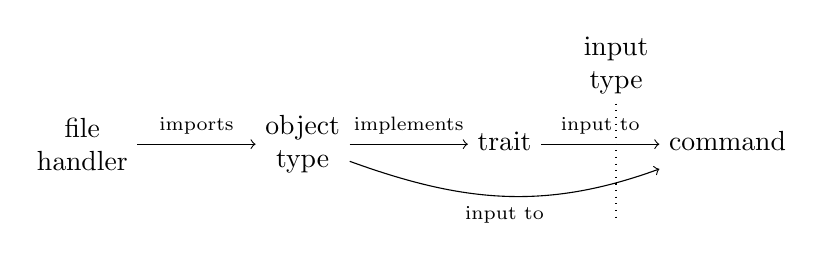
\begin{tikzpicture}
                \def\dx{1.5cm}
                \def\dy{1cm}
                \node (command) {command\strut};
    
                \node (trait) [left=\dx of command] {trait\strut};
    
                \node (objecttype) [left=\dx of trait, align=center] {object\\type};
    
                \node (filehandler) [left=\dx of objecttype, align=center] {file\\handler};
    
                \draw [->] (objecttype) to node[above, font=\scriptsize] {implements} (trait);
                \draw [->] (trait) to node[above, font=\scriptsize] {input to} (command);
    
                \draw [->, out=-20, in=200] (objecttype) to node[below, font=\scriptsize] {input to} (command);
    
                \draw [->] (filehandler) to node[above, font=\scriptsize] {imports} (objecttype);
    
                \node [align=center] (inputtype) at ($(trait)!0.5!(command)+(0,\dy)$) {input\\type};
                \draw [dotted] (inputtype) to ++(0,-2*\dy);
                
            \end{tikzpicture}\\
            \begin{tikzpicture}
                \def\dx{1.5cm}
                \def\dy{1cm}
                \node (command) {command\strut};  
    
                \node (objecttype) [left=\dx of trait, align=center] {object\\type};
    
                \node (filehandler) [left=\dx of objecttype, align=center] {file\\handler};
    
                \draw [<-, out=-20, in=200] (objecttype) to node[below, font=\scriptsize] {output of} (command);
    
                \draw [<-] (filehandler) to node[above, font=\scriptsize] {exported by} (objecttype);
    
                \node [align=center] (inputtype) at ($(trait)!0.5!(command)+(0,\dy)$) {output\\type};
                \draw [dotted] (inputtype) to ++(0,-2*\dy);
                
            \end{tikzpicture}
            \caption{Traits and object types in Ebi.}
            \label{fig:traits}
        \end{figure}
        
        
        \newgeometry{top=1mm,bottom=1mm,right=30mm,left=30mm}
        	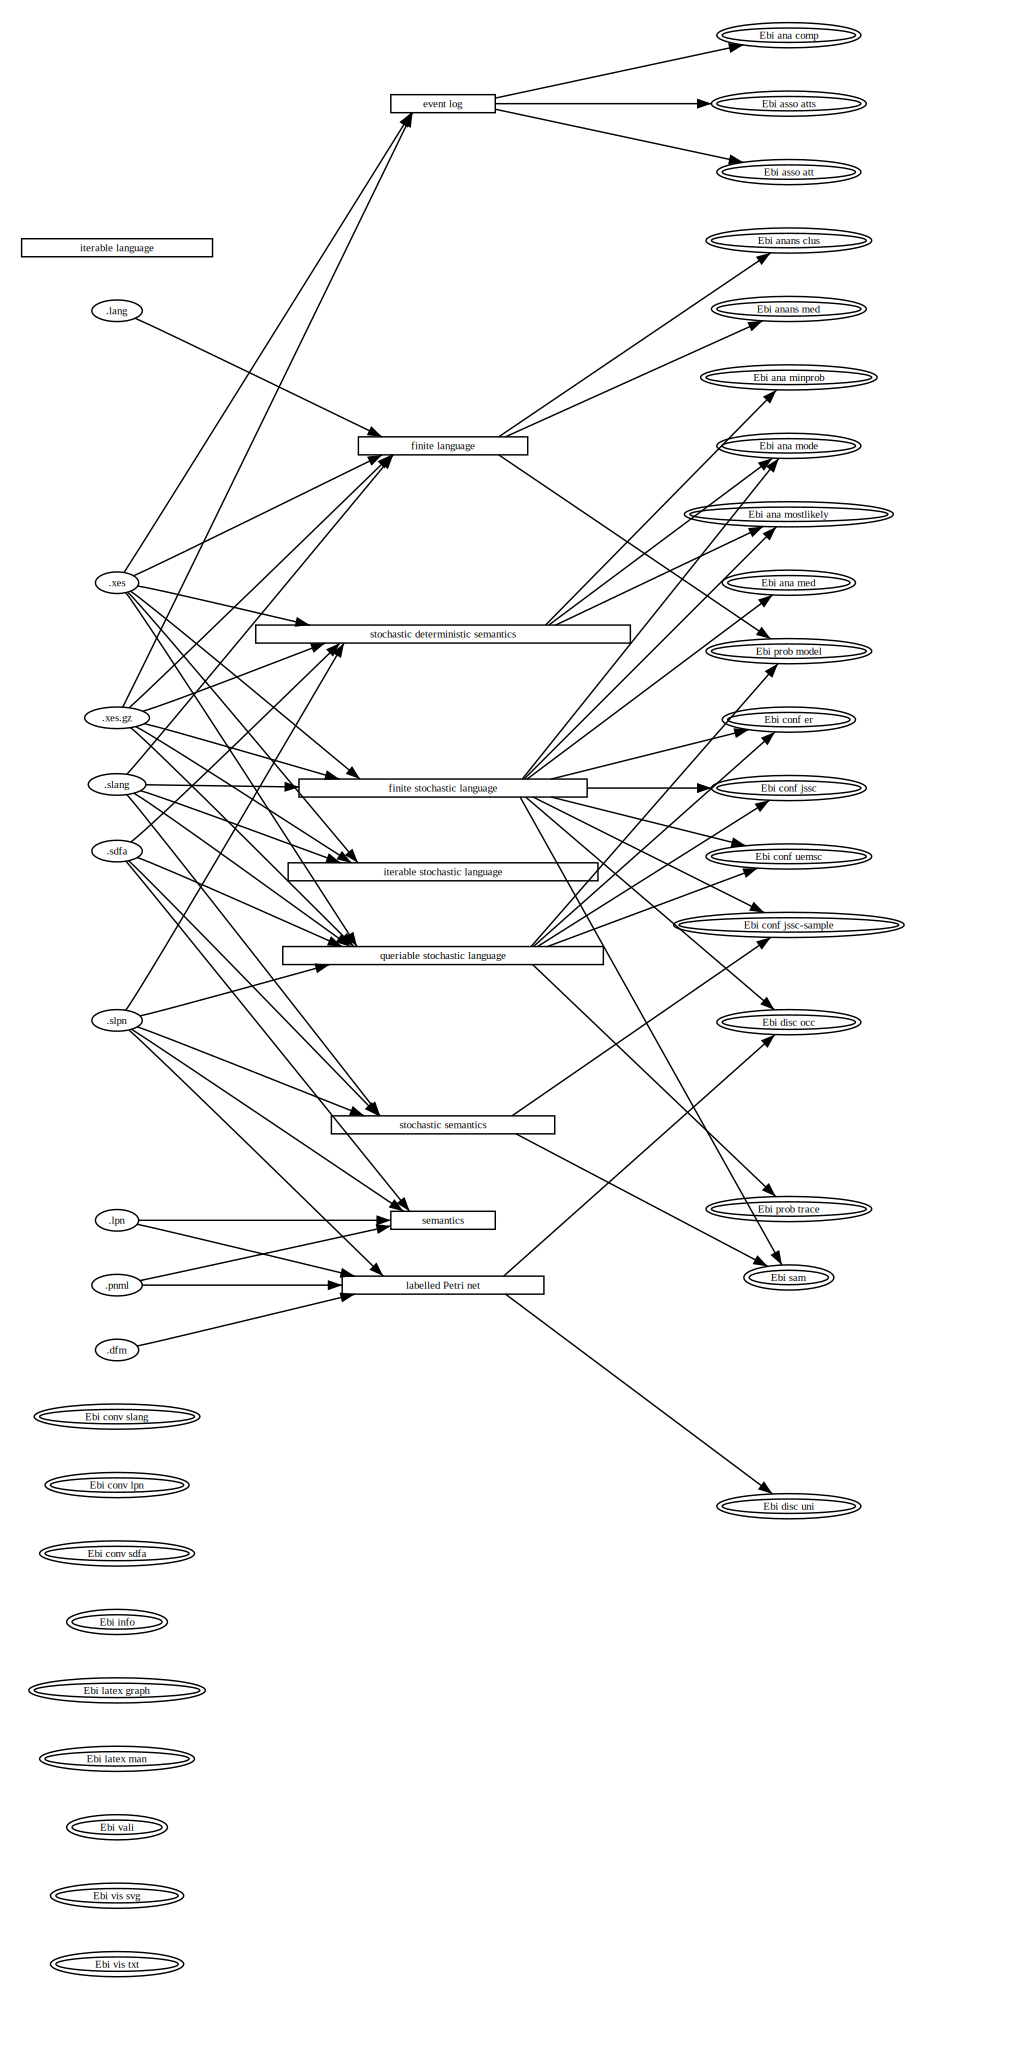
\includegraphics[width=0.5\linewidth]{graph}
        \restoregeometry
    
        \subsubsection{Command}
            A command is a function of Ebi that users can call.
            A command declares what types of inputs it needs and what type of output it generates. 
            Preferably, commands take traits as inputs rather than object types.
    
            Commands can circumvent the Ebi object handling on their inputs by declaring an \texttt{cli\_command} function, which gives direct access to the command line interface building process.
            This is for instance used in the \ebiCommand{validate} command, where we want to obtain the parsing error for a particular object type.
    
            The actual input for a command gets wrapped in the \texttt{EbiInput} enum, and the output must be wrapped in the \texttt{EbiOutput} enum.
            The Ebi machinery verifies whether the output of a command matches the declared output type at run time.
            
            Commands define a number of inputs, and for each input a list of acceptable types.
            However, these types need to be similar: a command cannot ask for either a file and a fraction, for instance.
    
            Ebi has the following commands:
            \ebicommandlist
    
        \subsubsection{Input type}
            An input type is a declaration of what a command needs as input.
            An input type can be:
            \begin{itemize}
                \item a trait;
                \item an object type;
                \item a basic data type such as fraction, integer or string;
                \item the ``any object" input type, which denotes that any object type will be accepted;
                \item a ``file handler", which indicates the (name of) a file handler (for instance used in the \ebiCommand{validate} command).
            \end{itemize}
    
            The actual input for a command gets wrapped in the \texttt{EbiInput} enum.
    
        \subsubsection{Trait}
            A ``trait" is like an interface: it provides some functions but does not say how these are implemented.
            For instance ``finite stochastic language" is a trait, which allows to iterate over traces and their probabilities, and to obtain the number of traces.
            Preferably, commands should require traits as inputs.

            Ebi has the following traits:
            \ebitraitlist
    
        \subsubsection{Object type}
            An object type is a struct or class.
            It is a specific implementation with a fixed data structure.
            The output of a command is an object of a specific object type.
            The input of a command rather not uses object types, but sometimes this is unavoidable.
            Objects are wrapped in an \texttt{EbiObject} enum to ensure type safety by the compiler.

            Ebi has the following object types:
            \ebiobjecttypelist
    
        \subsubsection{File handler}
            A file handler is an importer for a particular file format.
            In Ebi, a file handler defines how a file type is to be handled, and as which objects and traits it can be imported.
    
            Ebi has the following file handlers:
            \ebifilehandlerlist

    \subsection{Exact Computation}
        In Ebi, several computations are performed without rounding.
        To this end, it uses positive fractions: 
        $$\mathbb{Q} = \{ \frac{x}{y} \mid x, y \in \mathbb{N} \}$$
    
        Fractions are well-supported by standard libraries.
        Even for seemingly small fractions, the natural numbers that compose the fraction can get \emph{huge}.
        Therefore, simple 32 or 64 bit integers do not suffice for $x$ and $y$, and a large, unbounded, integer library is necessary.
    
        By default, Ebi uses exact arithmetic, unless it is disabled by a function explicitly.
        This can be done with \verb=Fraction::set_exact_globally(exact: bool)=.
        Please note that exact and approximate (double precision) arithmetic cannot be combined, thus functions should set this function as early as possible.

        \subsubsection{Square roots}
            Square roots can only be expressed in $\mathbb{N}$ or in $\mathbb{I}$.
            Thus, we need to represent square roots symbolically.
            For this, we use the following operations:
            \begin{align*}
                \frac{a}{b} ={}& \sqrt{\frac{a^2}{b^2}}\\
                \sqrt{a} \sqrt{b} ={}& \sqrt{a b}\\
                \frac{\sqrt{a}}{\sqrt{b}} ={}& \sqrt{\frac{a}{b}}
            \end{align*}
    
            Thus, we can represent all of these square root operations with the square root of a fractional number.

        \subsubsection{Logdiv}
            Logarithms can often not be expressed in $\mathbb{Q}$.
            For instance, $\log_2(3) \notin \mathbb{Q}$ is not a rational number.
            To perform computations exactly and to delay rounding to the very last moment, Ebi uses \emph{log division} objects.
            That is, computations that involve logarithms are performed symbolically in order not to have to evaluate the logarithm.
            
            A log division object ($\logdiv$) is a base-2 logarithm of a positive fraction, divided by a natural number:
            \begin{align*}
                \logdiv &{}\colon \mathbb{Q} \times \mathbb{N} \rightarrow \mathbb{I}\\
                \logdiv(\frac{a}{b}, c) &{}= \frac{\log(\frac{a}{b})}{c}\\
                &{}= \log \sqrt[\leftroot{-1}\uproot{2}\scriptstyle c]{\frac{a}{b}}
            \end{align*}

            \paragraph{From a fraction}
                Any non-negative fraction can be written as a $\logdiv$:
                \begin{align*}
                    \frac{a}{b} ={}& \frac{\log(2^a)}{b} \\
                    {}={}& \logdiv(\frac{2^a}{1}, b)
                \end{align*}
    
            \paragraph{Sum \& Difference}
                $\Logdiv$s are closed under addition:
                \begin{align*}
                    \logdiv(\frac{a}{b}, c) + \logdiv(\frac{d}{e}, f) = {}& 
                    \frac{\log(\frac{a}{b})}{c} + \frac{\log(\frac{d}{e})}{f}\\
                    {}={}& \frac{f\log(\frac{a}{b}) + c\log(\frac{d}{e})}{cf}\\
                    {}={}& \frac{\log(\frac{a^f}{b^f}) + \log(\frac{d^c}{e^c})}{cf}\\
                    {}={}& \frac{\log(\frac{a^f d^c}{b^f e^c})}{cf}\\
                    {}={}& \logdiv(\frac{a^f d^c}{b^f e^c}, cf)
                \end{align*}
                As $a$, $b$, $c$, $d$, $e$ and $f$ are all positive integers, the sum of two $\logdiv$s is also a $\logdiv$.
                Similarly, for subtraction:
                \begin{align*}
                    \logdiv(\frac{a}{b}, c) - \logdiv(\frac{d}{e}, f) = {}& 
                    \frac{\log(\frac{a}{b})}{c} - \frac{\log(\frac{d}{e})}{f}\\
                    {}={}& \frac{\log(\frac{a^f}{b^f}) - \log(\frac{d^c}{e^c})}{cf}\\
                    {}={}& \frac{\log(\frac{a^f}{b^f} / \frac{d^c}{e^c})}{cf}\\
                    {}={}& \logdiv(\frac{a^f e^c}{b^f d^c}, cf)\\
                \end{align*}
                As $a$, $b$, $d$ and $e$ are all positive integers, the difference between two $\logdiv$s is also a $\logdiv$.

            \paragraph{Additive identity (0)}
                The additive identity of $\logdiv$ is $\logdiv(\frac{1}{1}, 1) = 0$.
                
                While there are infinitely many $\logdiv$s that equal 0, such as $\logdiv(\frac{5}{5}, 100) = 0$, only a second argument of 1 guarantees that addition and subtraction work as intended.
                
            \paragraph{$n \log n$}
                Given a fraction $\frac{a}{b} \in \mathbb{Q}$, the value $\frac{a}{b} \log \frac{a}{b}$ can be represented by
                \begin{align*}
                    \frac{a}{b} \log \frac{a}{b} ={} & 
                    \frac{a \log(\frac{a}{b})}{b}\\
                    {}={}& \frac{\log(\frac{a^a}{b^a})}{b}\\
                    {}={}& \logdiv(\frac{a^a}{b^a}, b)\\
                \end{align*}

            \paragraph{Approximation}
                In order to provide readable results that can be used in other tools, at the end of the computation chain, $\logdiv$s need to be approximated to a fraction.
                To this end, we consider that:
                \begin{align*}
                    \logdiv(\frac{a}{b}, c) ={}& \frac{\log(\frac{a}{b})}{c}
                \end{align*}
    
                Thus, we need to compute $\log(q)$ with $q \in \mathbb{Q}$.
                As the libraries we use do not support computing logarithms on fractions with arbitrary large representations, we must implement this ourselves.

                \subparagraph{Taylor expansion}
                    Using Taylor expansion, we translate the approximation of the logarithm base 2 to $q$ to smaller and smaller values, until we end up with a $q' \leq 2$.
                    That is, we repeatedly divide $q$ by two and add one to the result, until $q$ drops below 2.
                    Then, we can approximate $\log_2(q)$ with a Taylor series on the natural logarithm\footnote{\url{https://en.wikipedia.org/wiki/Logarithm}}.
                    
                    \begin{align*}
                        \log(q) ={}& \begin{cases}
                            1 + \log(\frac{q}{2}) & \text{ if } q > 2\\ 
                            \frac{\ln(q)}{\ln(2)} & \text{ if } 0 < q \leq 2
                        \end{cases}\\
                        \ln(q) ={}& \sum_{k=1}^{\infty} (-1)^{k+1} \frac{(z-1)^k}{k} \text{ for } 0 < q \leq 2
                    \end{align*}
                    We then approximate $\ln(q)$ up until the terms become small enough for the required precision.

                \subparagraph{Bits}
                    As even standard multiplications are expensive for fractions, we need a more efficient strategy to bring the approximation to acceptable speed:
                    \begin{itemize}
                        \item If $\frac{a}{b} < \frac{1}{2}$:
                        \begin{align*}
                            \log(\frac{a}{b}) ={}& \log(a) - \log(b)\\
                            {}={}& -(\log(b) - \log(a))\\
                            {}={}& -\log(\frac{b}{a})
                        \end{align*}
                        In which $\frac{b}{a}$ is larger than 2.
    
                        Complexity: pointer swap.
                        
                        \item While $\frac{a}{b} > 1$:
                        \begin{align*}
                            \log(\frac{a}{b}) ={}& \begin{cases}
                                1 + \log(\frac{a}{2b}) & \text{if } a \text{ is odd}\\
                                1 + \log(\frac{a/2}{b}) & \text{if } a \text{ is even} \end{cases}
                        \end{align*}
                        Complexity: for each iteration a left or right bit shift plus a comparison (right bit shift).
                        
                        \item Then, $\frac{1}{2} < \frac{a}{b} < 1$.
                        %https://math.stackexchange.com/questions/1706939/approximation-log-2x
                        As $a$ and $b$ may be \emph{huge}, we cannot easily translate our fraction to a standard floating-point number.
                        Therefore, we use the following procedure to obtain as many digits as necessary for the required precision (where 3.3 bits yield one decimal):
                        \begin{align*}
                            \log(\frac{a}{b})_n ={}& \begin{cases}
                                1 & \text{if } a = b\\
                                \log(\frac{a^2}{2 b^2})_{n+1} - \frac{1}{2^n} & \text{if } \frac{a^2}{b^2} > 2 \qquad \text{report a binary } 1\\
                                \log(\frac{a^2}{b^2})_{n+1} & \text{otherwise} \qquad \text{report a binary } 0\\
                            \end{cases}
                        \end{align*}
                        In which $n$ denotes the iteration.
    
                        Complexity: two multiplications and at most one bit shift per bit precision.
                        As multiplications are prohibitively expensive, and squaring roughly doubles the number of bits each iteration, we truncate $a$ and $b$ by the same number of bit-shifts every iteration, such that in each number enough bits are left.
                    \end{itemize}

        \subsubsection{RootLogDiv}
            A RootLogDiv is the following:
            \begin{align*}
                \text{RootLogDiv}(\frac{a}{b},c) ={}& \sqrt{\logdiv(\frac{a}{b}, c)}\\
                {}={}& \sqrt{\frac{\log\frac{a}{b}}{c}}& 
            \end{align*}

            There is an option to perform the 1- operation on a RootLogDiv.
        
    \section{Entropic Relevance}
    \label{sec:er}
        Entropic relevance is computed as follows:
        
        \begin{definition}[Entropic Relevance~\cite{DBLP:journals/is/AlkhammashPMG22}]
            \label{def:ER}
                Let $L$ be a finite stochastic language and let $M$ be a queriable stochastic langauge.
                Let $\Lambda$ be the set of all activities appearing in the traces of $L$.
                Then, the \emph{entropic relevance ($\entrel$) of $M$ to $L$} is defined as follows: 
                \begin{align*}
                    \entrel(L, M) ={}& H_0\left(\sum_{\sigma \in \bar{L},\, M(\sigma)>0}{L(\sigma)}\right) + 
                    \sum_{\sigma \in \bar{L}}L(\sigma) J(\sigma, M)\\
                    J(\sigma, M) ={}& \begin{cases}
                    -\log_2 M(\sigma) & M(\sigma) > 0\\
                    (1+|\sigma|) \log_2 (1 + |\Lambda|)) & \text{otherwise}
                    \end{cases}\\
                    H_0(x) ={}& -x \log_2{x} - (1-x) \log_2{(1-x)} \text{ with } H_0(0) = H_0(1) = 0 &\\
                \end{align*}       
            \end{definition}
            
    \bibliographystyle{plain}
    \bibliography{bibliography}

    \printindex
\end{document}